\documentclass[border=6pt]{standalone}
\usepackage{amsmath,amssymb}
\usepackage{tikz}
\usepackage{newtxtext,newtxmath}
\usetikzlibrary{arrows.meta,positioning,fit,backgrounds,calc}

% Pure white background + IEEE Okabe-Ito colorblind-safe muted palette
\definecolor{SlateBorder}{HTML}{0072B2}
\definecolor{SlateFill}{HTML}{EFF6FC}
\definecolor{AmberBorder}{HTML}{D55E00}
\definecolor{AmberFill}{HTML}{FFF6EC}
\definecolor{BackboneBorder}{HTML}{1E293B}
\definecolor{BackboneFill}{HTML}{F8FAFC}
\definecolor{Head1Border}{HTML}{B45309}
\definecolor{Head1Fill}{HTML}{FFFBEB}
\definecolor{Head2Border}{HTML}{9D174D}
\definecolor{Head2Fill}{HTML}{FDF2F8}
\definecolor{CbfBorder}{HTML}{047857}
\definecolor{CbfFill}{HTML}{ECFDF5}
\definecolor{ContainerBorder}{HTML}{475569}
\definecolor{ContainerFill}{HTML}{FCFDFF}
\definecolor{TextDark}{HTML}{0F172A}
\definecolor{TextSub}{HTML}{334155}

\begin{document}
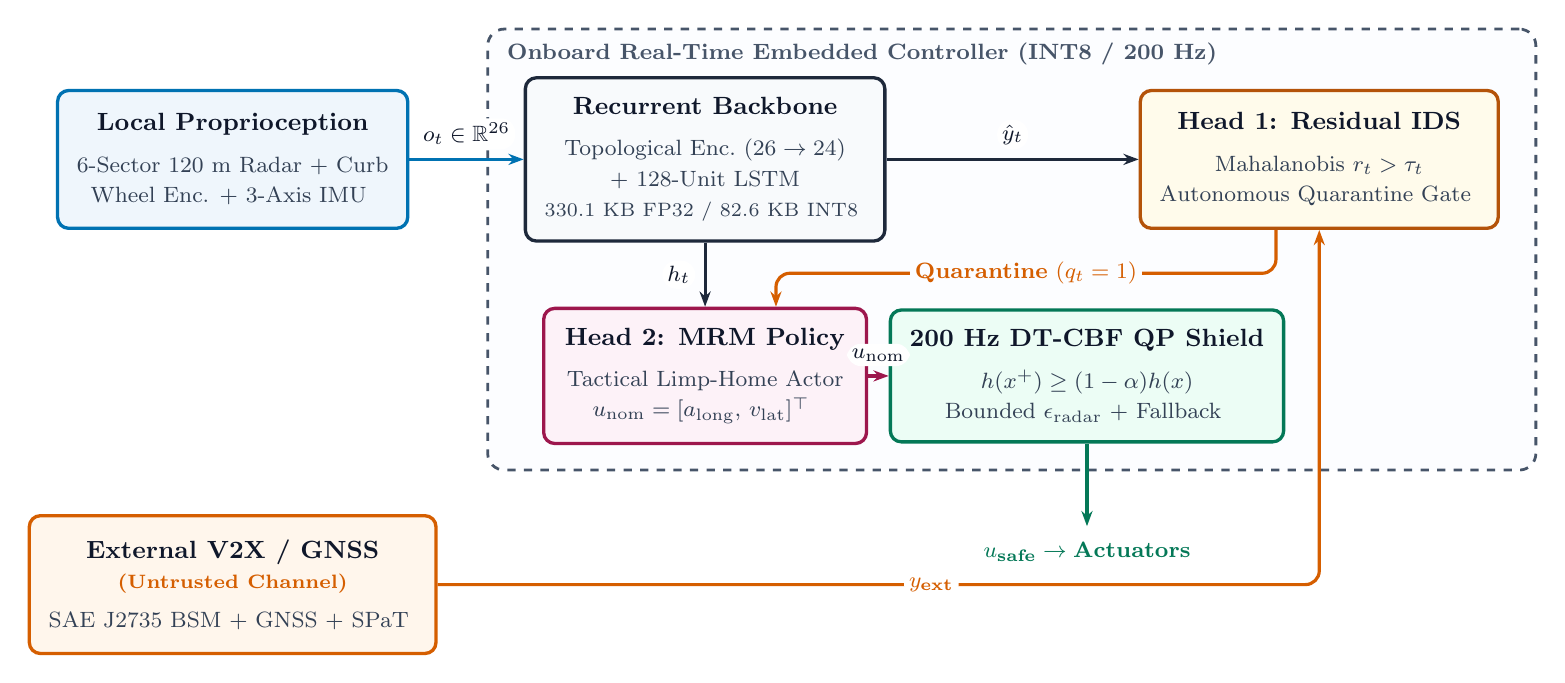
\begin{tikzpicture}[
    font=\rmfamily,
    >=Stealth,
    node distance=1.4cm,
    box/.style={
        draw=#1,
        line width=1.2pt,
        rounded corners=4pt,
        align=center,
        inner sep=7pt,
        text=TextDark
    },
    arr/.style={
        -{Stealth[length=5.5pt,width=4pt]},
        line width=1.15pt,
        rounded corners=5pt
    },
    lbl/.style={
        font=\footnotesize,
        fill=white,
        inner sep=1.8pt,
        text=TextDark
    }
]

% Left column: Trusted local proprioception (top-left) & Untrusted external V2X/GNSS (bottom-left)
\node[box=SlateBorder, fill=SlateFill, minimum width=4.0cm, minimum height=1.75cm] (local) at (-6.0, 2.5) {%
    \textbf{\small Local Proprioception}\\[3pt]
    \footnotesize\color{TextSub}6-Sector $120\text{ m}$ Radar + Curb\\[-1pt]
    \footnotesize\color{TextSub}Wheel Enc. + 3-Axis IMU
};

\node[box=AmberBorder, fill=AmberFill, minimum width=4.0cm, minimum height=1.75cm] (external) at (-6.0, -2.9) {%
    \textbf{\small External V2X / GNSS}\\[-1pt]
    \textbf{\scriptsize\color{AmberBorder}(Untrusted Channel)}\\[2pt]
    \footnotesize\color{TextSub}SAE J2735 BSM + GNSS + SPaT
};

% Onboard blocks: Top track (Backbone -> Head 1) and Middle track (Head 2 -> DT-CBF)
\node[box=BackboneBorder, fill=BackboneFill, minimum width=4.4cm, minimum height=1.85cm] (backbone) at (0.0, 2.5) {%
    \textbf{\small Recurrent Backbone}\\[3pt]
    \footnotesize\color{TextSub}Topological Enc.\ ($26 \to 24$)\\[-1pt]
    \footnotesize\color{TextSub}$+$\ 128-Unit LSTM\\[-1pt]
    \scriptsize\color{TextSub}$330.1\text{ KB}$ FP32 / $82.6\text{ KB}$ INT8
};

\node[box=Head1Border, fill=Head1Fill, minimum width=4.1cm, minimum height=1.75cm] (head1) at (7.8, 2.5) {%
    \textbf{\small Head 1: Residual IDS}\\[3pt]
    \footnotesize\color{TextSub}Mahalanobis $r_t > \tau_t$\\[-1pt]
    \footnotesize\color{TextSub}Autonomous Quarantine Gate
};

\node[box=Head2Border, fill=Head2Fill, minimum width=4.1cm, minimum height=1.65cm] (head2) at (0.0, -0.25) {%
    \textbf{\small Head 2: MRM Policy}\\[3pt]
    \footnotesize\color{TextSub}Tactical Limp-Home Actor\\[-1pt]
    \footnotesize\color{TextSub}$u_{\text{nom}} = [a_{\text{long}},\, v_{\text{lat}}]^\top$
};

\node[box=CbfBorder, fill=CbfFill, minimum width=4.1cm, minimum height=1.65cm] (cbf) at (4.85, -0.25) {%
    \textbf{\small 200 Hz DT-CBF QP Shield}\\[3pt]
    \footnotesize\color{TextSub}$h(x^+) \ge (1-\alpha)h(x)$\\[-1pt]
    \footnotesize\color{TextSub}Bounded $\epsilon_{\text{radar}}$ + Fallback
};

% Subtle dashed embedded controller container separating onboard execution from untrusted external feeds
\begin{scope}[on background layer]
    % Force pure #FFFFFF page backdrop across full bounding box
    \node[
        draw=ContainerBorder,
        dashed,
        line width=1.0pt,
        rounded corners=6pt,
        fill=ContainerFill,
        fit=(backbone)(head1)(head2)(cbf),
        inner xsep=13pt,
        inner ysep=13pt,
        yshift=4pt,
        label={[anchor=north west, font=\footnotesize\bfseries, text=ContainerBorder, xshift=4pt, yshift=-2pt]north west:Onboard Real-Time Embedded Controller (INT8 / 200 Hz)}
    ] (controller) {};
\end{scope}

% 1. Local Proprioception -> Recurrent Backbone (straight horizontal)
\draw[arr, SlateBorder] (local.east) -- node[lbl, above=3pt] {$o_t \in \mathbb{R}^{26}$} (backbone.west);

% 2. Recurrent Backbone -> Head 1: Residual IDS (straight horizontal)
\draw[arr, BackboneBorder] (backbone.east) -- node[lbl, above=3pt] {$\hat{y}_t$} (head1.west);

% 3. Recurrent Backbone -> Head 2: MRM Policy (straight down)
\draw[arr, BackboneBorder] (backbone.south) -- node[lbl, left=3pt] {$h_t$} (head2.north);

% 4. Head 1 -> Head 2: Quarantine (clean orthogonal route inside open middle corridor, no crossings)
\draw[arr, AmberBorder] ([xshift=-0.55cm]head1.south) -- ++(0, -0.55) -| node[lbl, pos=0.25, fill=ContainerFill] {\color{AmberBorder}\textbf{Quarantine} ($q_t=1$)} ([xshift=0.9cm]head2.north);

% 5. Head 2 -> 200 Hz DT-CBF QP Safety Shield (straight horizontal)
\draw[arr, Head2Border] (head2.east) -- node[lbl, above=3pt] {$u_{\text{nom}}$} (cbf.west);

% 6. 200 Hz DT-CBF -> Actuators (straight down out of controller container, above bottom external track)
\draw[arr, CbfBorder] (cbf.south) -- ++(0, -1.05) node[below=2pt, font=\footnotesize\bfseries, text=CbfBorder] {$u_{\text{safe}} \to \text{Actuators}$};

% 7. External V2X / GNSS -> Head 1 (horizontal along bottom track, clean -| orthogonal bend right into Head 1)
\draw[arr, AmberBorder] (external.east) -| node[lbl, pos=0.28, text=AmberBorder] {\textbf{$y_{\text{ext}}$}} (head1.south);

\end{tikzpicture}
\end{document}
